\chapter{Implementazione}
\label{cha:implementazione}

In questo capitolo viene mostrata l'implementazione della pipeline dati sviluppata durante
il tirocinio. Dopo aver descritto il contesto e le tecnologie adottate nei capitoli precedenti, qui l’attenzione si sposta sugli aspetti pratici della realizzazione.
L’obiettivo principale è stato quello di trasformare un unico script monolitico in un sistema modulare e automatizzato, basato su Apache Airflow e containerizzato tramite Docker. La nuova architettura non solo consente di programmare e monitorare l’esecuzione dei workflow, ma integra anche strumenti di osservabilità, rendendo possibile analizzare in tempo reale lo stato delle esecuzioni e le risorse utilizzate.

Nel corso del capitolo verranno quindi analizzati:


\begin{itemize}
    \item la definizione del DAG e delle task che lo compongono, con l’illustrazione delle modifiche apportate agli script originari per adattarli al nuovo contesto;
    \item la containerizzazione del sistema, descrivendo nel dettaglio il Dockerfile e il file docker-compose.yml;
    \item l’infrastruttura di monitoraggio, con le configurazioni di StatsD, Prometheus e Grafana;
    \item l’integrazione dei diversi componenti e le modalità di deploy dell’applicazione.
\end{itemize}

In questo modo si vuole mostrare il percorso seguito per passare da una soluzione monolitica e difficile da mantenere a un’infrastruttura completa, affidabile, automatizzata e osservabile.

\begin{figure}[ht]
    \centering
    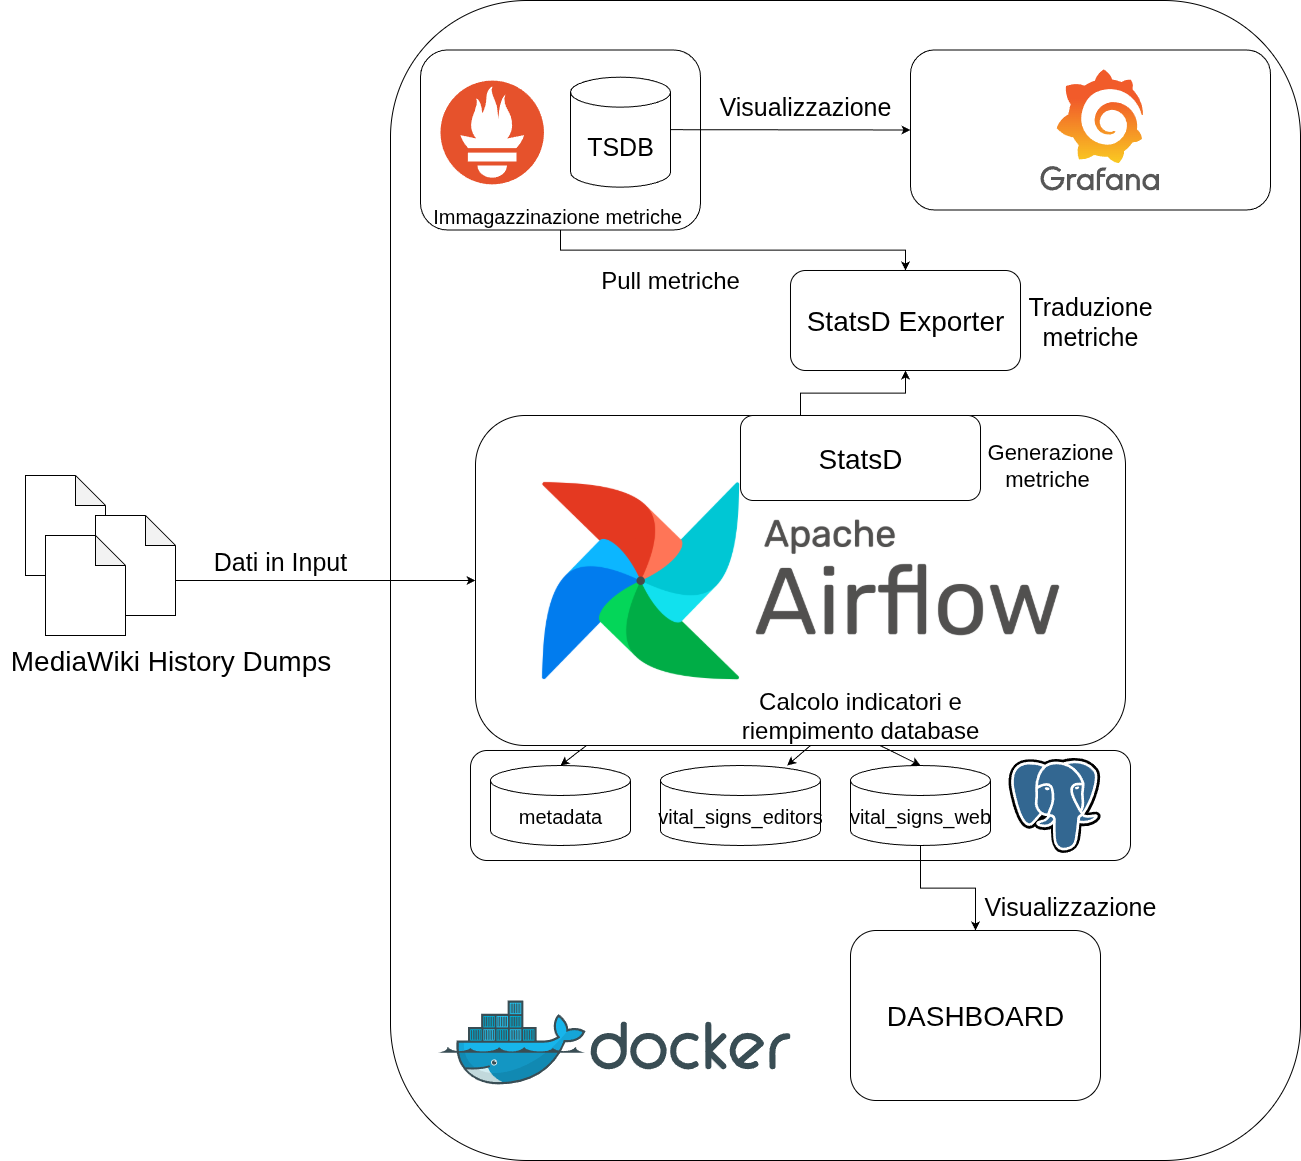
\includegraphics[width=\textwidth]{img/vital-signs-pipeline.drawio.png}
    \caption{Schema logico dell'architettura del sistema}
    \label{fig:architettura_sistema}
\end{figure}

\section{DAG e script}
\label{sec:dag_script}

Come introdotto nella Sezione~\ref{sec:airflow}, il Directed Acyclic Graph (DAG) è lo strumento con cui Apache Airflow permette di modellare un workflow come un insieme di task con relazioni di dipendenza.

Nel progetto ho definito il DAG vital\_signs, contenuto nel file vital\_signs\_dag.py all’interno della cartella dags/. Questo DAG ha il compito di processare i dati provenienti dai MediaWiki History Dumps, eseguendo diversi calcoli su di essi e popolando progressivamente due database distinti: prima quello degli editors, che raccoglie le metriche derivate dai dump, e successivamente quello web, in cui vengono calcolati e salvati i vital signs a partire dalle metriche estratte.

Vediamo ora come è stato definito il DAG, le sue caratteristiche principali e come sono stati adattati gli script esistenti per funzionare in questo nuovo contesto.

\newpage

\begin{lstlisting}[language=Python, caption=Definizione del DAG in Airflow, label=lst:dag_definition]
# Import delle librerie necessarie e funzioni di supporto
with DAG(
    dag_id='vital_signs',
    default_args={
        'owner': 'andrea_denina',
        'depends_on_past': False,
        'start_date': datetime(2025, 4, 15),
        'retries': 1,
        'retry_delay': timedelta(minutes=5),
    },
    description='Compute Community Health Metrics (CHM) 
    from MediaWiki History dumps for multiple languages',
    schedule_interval='0 0 10 * *',
    catchup=False,
    max_active_runs=1
) as dag:
    # Definizione dei task
\end{lstlisting}

Il codice in lst. \ref{lst:dag_definition} mostra la definizione del DAG vital\_signs e i suoi parametri principali.

In particolare:

\begin{itemize}
    \item \textbf{dag\_id}: assegna un identificativo univoco al DAG, in questo caso vital\_signs.
    \item \textbf{default\_args}: raccoglie i parametri comuni a tutte le task, come l'owner, la data di inizio, il numero di retry e il ritardo tra un tentativo e l'altro.
    \item \textbf{start\_date}: definisce la data a partire dalla quale Airflow può schedulare le esecuzioni del DAG.
    \item \textbf{schedule\_interval}: stabilisce la frequenza di esecuzione. È stata scelta un'espressione cron che fa partire il DAG ogni 10 del mese, in linea con le tempistiche di pubblicazione dei dump.
    \item \textbf{catchup}: impostato a False, evita che al primo avvio il DAG tenti di recuperare retroattivamente tutte le esecuzioni mancate dal start\_date.
    \item \textbf{max\_active\_runs}: limita il numero di esecuzioni contemporanee del DAG a uno, per prevenire conflitti nell'accesso ai dati.
\end{itemize}


\subsection{Struttura delle task}
\label{subsec:struttura_task}

Nel DAG vital\_signs le task sono tutte implementate come PythonOperator,
quindi ciascuna invoca uno script Python specifico.
La pipeline è delimitata da due sentinelle logiche, start ed end (entrambi EmptyOperator), fra le quali si sviluppa il flusso di elaborazione.
Subito dopo l’avvio, la task create\_dbs prepara l’ambiente applicativo creando e inizializzando le tabelle dei due database coinvolti (editors e web).
A questo punto il DAG si ramifica per lingua (in base a wikilanguagecodes) e per ogni edizione linguistica vengono eseguiti in sequenza tre step:
\textless code\textgreater\_process\_dump per estrarre e caricare le metriche dai MediaWiki History Dumps nel DB degli editor,
\textless code\textgreater\_calc\_flags per calcolare i flag/profili degli editor,
\textless code\textgreater\_calc\_streaks per derivare le streak di attività.

Terminata la fase per lingua sul database vital\_signs\_editors, una fase cross wiki (calc\_primary\_language) calcola la lingua primaria degli utenti a partire dalle metriche calcolate nelle precedenti fasi.
Infine, avviene una seconda ramificazione per lingua dove, con \textless code\textgreater\_calc\_vs, si computano i vital signs e si popolano le tabelle del database  vital\_signs\_web a partire dalle metriche già consolidate.
L’intera catena è vincolata da dipendenze esplicite (\textgreater \textgreater) che assicurano l’ordine corretto; inoltre, ogni task utilizza callback di logging di esito (on\_success\_callback, on\_failure\_callback) per tracciare in modo uniforme completamenti e fallimenti delle esecuzioni.
In questo modo il DAG rimane leggibile e modulare: ogni task incapsula un passaggio ben definito e l’orchestrazione di Airflow garantisce una progressione deterministica dall’ingestione dei dump fino alla produzione dei vital signs.


\begin{lstlisting}[language=Python, caption={Esempio di definizione di una task e dipendenze del DAG}, label=lst:dag_tasks]
start = EmptyOperator(task_id='start', dag=dag)
end = EmptyOperator(task_id='end', dag=dag)

create_dbs_task = PythonOperator(
    task_id="create_dbs",
    python_callable=create_db,
    dag=dag,
    op_args=[wikilanguagecodes],
    on_success_callback=log_task_end,
    on_failure_callback=log_task_failure,
)

...

start >> create_dbs_task >> editors_db_group \
      >> primary_language_task >> web_db_group >> end
\end{lstlisting}

Nel codice in lst. \ref{lst:dag_tasks} è mostrato un esempio di definizione di una task (create\_dbs) e la struttura delle dipendenze del DAG.
Come si può notare la task chiama la funzione create\_db, definita in un file nella cartella scripts/ e importata come una libreria.
Il parametro op\_args permette di passare argomenti alla funzione, in questo caso la lista delle lingue da processare.
\paragraph{}
Dopo aver descritto la struttura complessiva del DAG, è utile analizzare nel dettaglio le singole task che lo compongono.
Per rendere la pipeline più modulare e leggibile, lo script originario è stato suddiviso in sei parti principali, ciascuna delle quali è associata a una specifica fase del flusso e implementata come task indipendente. In questo modo ogni passaggio è incapsulato in una funzione python separata ed eseguito tramite un PythonOperator.

Nelle sottosezioni che seguono verranno illustrate le task una ad una, evidenziandone lo scopo e la logica implementativa.
Infine, verrà presentato un esempio di refactoring relativo al calcolo della lingua primaria degli editor, dove l’utilizzo della libreria Pandas ha permesso di migliorare leggibilità ed efficienza del codice.
\subsection{Task create\_dbs}
\label{subsec:create_dbs}

La prima task del DAG è \texttt{create\_dbs}, responsabile dell’inizializzazione dei database utilizzati dalla pipeline. 
Si tratta di un passo preliminare che assicura la presenza e la corretta struttura delle tabelle necessarie sia per il database degli \emph{editors} sia per quello dei \emph{vital signs}. 
La task è implementata come \texttt{PythonOperator} e chiama la funzione \texttt{create\_db}, definita in un file (\texttt{create\_db.py}) nella cartella \texttt{scripts/}.

Lo script utilizza la libreria \texttt{SQLAlchemy} per gestire le connessioni ai due database (tramite le stringhe di connessione definite in \texttt{config.py}). 
Per ciascuna lingua in \texttt{wikilanguagecodes} vengono create due tabelle nel database \texttt{vital\_signs\_editors}:

\begin{itemize}
    \item \texttt{<langcode>wiki\_editors}, che raccoglie le informazioni anagrafiche e di profilo degli editor.
    \item \texttt{<langcode>wiki\_editor\_metrics}, che memorizza le metriche derivate dai dump a livello di utente e mese.
\end{itemize}

Infine, nel database \texttt{vital\_signs\_web} viene inizializzata la tabella \texttt{vital\_signs\_metrics}, che conterrà gli indicatori aggregati calcolati nelle fasi successive. 

Il codice seguente mostra le definizioni SQL semplificate delle tre tabelle principali:

\newpage 

\begin{lstlisting}[language=SQL, caption={Definizione delle tabelle create dalla task create\_dbs}, label=lst:create_dbs_tables, basicstyle=\scriptsize\ttfamily]
-- Tabella <langcode>wiki_editors
CREATE TABLE IF NOT EXISTS <langcode>wiki_editors (
    user_id INTEGER,
    user_name TEXT PRIMARY KEY,
    bot TEXT,
    user_flags TEXT,
    highest_flag TEXT,
    highest_flag_year_month TEXT,
    gender TEXT,
    primarybinary INTEGER,
    primarylang TEXT,
    edit_count INTEGER,
    primary_ecount INTEGER,
    totallangs_ecount INTEGER,
    primary_year_month_first_edit TEXT,
    primary_lustrum_first_edit TEXT,
    numberlangs INTEGER,
    registration_date TEXT,
    year_month_registration TEXT,
    first_edit_timestamp TEXT,
    year_month_first_edit TEXT,
    year_first_edit TEXT,
    lustrum_first_edit TEXT,
    survived60d TEXT,
    last_edit_timestamp TEXT,
    year_last_edit TEXT,
    lifetime_days INTEGER,
    days_since_last_edit INTEGER
);

-- Tabella <langcode>wiki_editor_metrics
CREATE TABLE IF NOT EXISTS <langcode>wiki_editor_metrics (
    user_id INTEGER,
    user_name TEXT,
    abs_value TEXT,
    rel_value REAL,
    metric_name TEXT,
    year_month TEXT,
    timestamp TEXT,
    PRIMARY KEY (user_id, metric_name, year_month, timestamp)
);

-- Tabella vital_signs_metrics
CREATE TABLE IF NOT EXISTS vital_signs_metrics (
    langcode TEXT,
    year_year_month TEXT,
    year_month TEXT,
    topic TEXT,
    m1 TEXT,
    m1_calculation TEXT,
    m1_value TEXT,
    m2 TEXT,
    m2_calculation TEXT,
    m2_value TEXT,
    m1_count FLOAT,
    m2_count FLOAT,
    PRIMARY KEY (langcode, year_year_month, year_month, topic, 
                m1, m1_calculation, m1_value, 
                m2, m2_calculation, m2_value)
);
\end{lstlisting}

In sintesi, le prime due tabelle costituiscono il livello “di base” per ciascuna lingua, registrando rispettivamente i dati anagrafici degli editor e le metriche puntuali calcolate dai dump. 
La terza tabella rappresenta invece il livello “aggregato” e contiene i \emph{vital signs}, calcolati a partire dalle metriche di base e organizzati in modo idempotente grazie a una chiave primaria composta che impedisce inserimenti duplicati.  

Al termine dell’esecuzione di questa task l’ambiente risulta pronto per accogliere i dati estratti dai dump e per memorizzare i risultati delle analisi successive.

\subsection{Task \textless langcode\textgreater\_process\_dump}
\label{subsec:process_dump}

La task \texttt{<langcode>\_process\_dump} è la più impegnativa del DAG in termini computazionali. 
Per ogni edizione linguistica viene creata una task dedicata che legge i MediaWiki History Dumps compressi (\texttt{.bz2}) e ne estrae i dati rilevanti sugli editor, trasformando i record grezzi in metriche strutturate da salvare nel database \texttt{vital\_signs\_editors}. 
Questa impostazione consente al DAG di scalare su più comunità linguistiche semplicemente modificando la lista \texttt{wikilanguagecodes}, da cui Airflow genera dinamicamente le task.

\begin{table}[h]
\centering
\scriptsize
\begin{tabular}{|c|l|l|p{8cm}|}
\hline
\textbf{Idx} & \textbf{Variabile} & \textbf{Tipo} & \textbf{Descrizione} \\
\hline
1  & \texttt{event\_entity} & string & Entità dell’evento: \emph{revision}, \emph{user} o \emph{page}. \\
2  & \texttt{event\_type} & string & Tipo di evento: \emph{create}, \emph{move}, \emph{delete}, ecc. \\
3  & \texttt{event\_timestamp} & string & Timestamp in cui si è verificato l’evento. \\
5  & \texttt{event\_user\_id} & bigint & ID dell’utente che ha generato l’evento (null se anonimo o revision-deleted). \\
7  & \texttt{event\_user\_text} & string & Username corrente dell’utente (IP se anonimo). \\
11 & \texttt{event\_user\_groups} & array \textless string \textgreater & Gruppi correnti a cui appartiene l’utente. \\
13 & \texttt{event\_user\_is\_bot\_by} & array \textless string \textgreater & Informazioni sullo stato di bot (nome o gruppo). \\
17 & \texttt{event\_user\_is\_anonymous} & boolean & Indica se l’utente è anonimo. \\
20 & \texttt{event\_user\_registration\_timestamp} & string & Timestamp di registrazione dell’utente (da tabella user). \\
21 & \texttt{event\_user\_creation\_timestamp} & string & Timestamp di creazione account (da logging). \\
22 & \texttt{event\_user\_first\_edit\_timestamp} & string & Timestamp del primo edit dell’utente. \\
23 & \texttt{event\_user\_revision\_count} & bigint & Numero cumulativo di revisioni effettuate fino all’evento (include l’evento stesso). \\
30 & \texttt{page\_namespace} & int & Namespace corrente della pagina. \\
38 & \texttt{user\_id} & bigint & Identificativo dell’utente (in eventi di tipo user). \\
40 & \texttt{user\_text} & string & Username o indirizzo IP corrente (in eventi di tipo user). \\
44 & \texttt{user\_groups} & array \textless string \textgreater & Gruppi correnti dell’utente (in eventi di tipo user). \\
\hline
\end{tabular}
\caption{Variabili dei MediaWiki History Dumps utilizzate dalla pipeline con relativi indici, tipi e descrizioni.}
\label{tab:dump_variables_selected}
\end{table}


I principali dati estratti e rielaborati sono i seguenti:

\begin{itemize}
  \item \textbf{Identificazione dell’utente}: vengono considerati solo eventi con \texttt{event\_user\_id} valido e non anonimo (\texttt{event\_user\_is\_anonymous = False}). A ciascun utente vengono associati username (\texttt{event\_user\_text}), flag e stato (bot/non-bot).
  \item \textbf{Informazioni temporali}: da \texttt{event\_timestamp} si derivano date di registrazione, primo edit, ultimo edit, anno e mese dei contributi.
  \item \textbf{Flag e gruppi}: dalle variabili \texttt{event\_user\_groups} e dagli eventi di tipo \texttt{altergroups} vengono ricostruite le modifiche di gruppo nel tempo. Questi eventi sono salvati in \texttt{wiki\_editor\_metrics} con metriche \texttt{granted\_flag} e \texttt{removed\_flag}.
  \item \textbf{Monthly edits}: per ogni utente e mese viene calcolato il numero di revisioni (\texttt{revision\_id}) effettuate, salvato come metrica \texttt{monthly\_edits}.
  \item \textbf{Namespace edits}: il campo \texttt{page\_namespace} distingue i contributi nei namespace di coordinamento (4, 12) e tecnici (8, 10), salvati rispettivamente come \texttt{monthly\_edits\_coordination} e \texttt{monthly\_edits\_technical}.
  \item \textbf{Metriche di sopravvivenza}: a partire dal \texttt{event\_user\_first\_edit\_timestamp} vengono calcolate le soglie di attività entro 24 ore, 7 giorni, 30 giorni e 60 giorni dal primo edit (\texttt{edit\_count\_24h}, \texttt{edit\_count\_7d}, \texttt{edit\_count\_30d}, \texttt{edit\_count\_60d}). Tali metriche servono come base per la successiva analisi di retention.
  \item \textbf{Caratteristiche anagrafiche e storiche}: per ogni utente vengono salvati attributi quali data di registrazione, anno/mese del primo e ultimo edit, lustro di ingresso (\texttt{lustrum\_first\_edit}), numero di giorni di vita dell’account (\texttt{lifetime\_days}) e giorni trascorsi dall’ultimo edit (\texttt{days\_since\_last\_edit}). È inoltre marcato se l’utente è sopravvissuto almeno 60 giorni (\texttt{survived60d}).
\end{itemize}

I risultati vengono infine inseriti in due tabelle distinte:
\begin{itemize}
  \item \texttt{<langcode>wiki\_editor\_metrics}, che raccoglie le metriche mensili (edits totali, edits per namespace) e le misure di sopravvivenza (edit\_count\_*). 
  \item \texttt{<langcode>wiki\_editors}, che conserva le informazioni anagrafiche e di attività degli utenti (flag, lingua primaria, date di registrazione/attività, edit count complessivo, ecc.).
\end{itemize}

Tutti gli inserimenti avvengono in modalità idempotente (\texttt{ON CONFLICT DO NOTHING} o \texttt{DO UPDATE}), in modo da evitare duplicazioni quando la pipeline viene rieseguita sugli stessi dump. 
In questo modo la task produce un dataset consistente e normalizzato, da cui le fasi successive del DAG (\texttt{calc\_flags}, \texttt{calc\_streaks}, \texttt{calc\_vs}) possono derivare i \emph{vital signs}.


\subsection{Task \textless langcode\textgreater\_calc\_flags}
\label{subsec:calc_flags}

La task \textless langcode\textgreater\_calc\_flags ha lo scopo di analizzare i flag assegnati agli editor
e individuare per ciascun utente quello di rango più elevato,
salvandolo nella tabella degli editors.
Per ogni edizione linguistica viene generata una task dedicata che prende come input il codice della lingua e utilizza i dati prodotti dalla fase precedente e salvati nel database \texttt{vital\_signs\_editors}.

Lo script associato alla task \texttt{calc\_flags} (\texttt{calculate\_editors\_flag}) si occupa di determinare, per ciascun utente, il flag più rilevante ricevuto durante la sua attività. In un primo passaggio vengono contati i flag presenti tra tutti gli editor, così da costruire un dizionario di supporto. Successivamente è definita una gerarchia di priorità (\emph{flag ranks}) che assegna un valore crescente ai diversi flag: dai più comuni, come \texttt{confirmed}, fino a quelli di maggiore responsabilità, come \texttt{steward} o \texttt{founder}.

Per ogni editor viene quindi valutata la lista dei flag posseduti e viene individuato quello con rango massimo, salvato nel campo \texttt{highest\_flag} della tabella \texttt{wiki\_editors}. Nel caso in cui più flag abbiano lo stesso livello, viene selezionato quello più diffuso all’interno della comunità. Lo script aggiorna inoltre il campo \texttt{highest\_flag\_year\_month}, basandosi sugli eventi di concessione flag (\texttt{granted\_flag}) registrati in \texttt{wiki\_editor\_metrics}, così da associare il flag principale al momento in cui è stato effettivamente ottenuto. Infine, viene gestito il caso specifico degli utenti che hanno ricevuto un flag di tipo \texttt{bot}, aggiornando opportunamente il campo \texttt{bot} nella tabella degli editor.

In questo modo la task arricchisce il profilo di ciascun editor con informazioni sul ruolo più significativo ricoperto nella comunità e sul momento in cui tale ruolo è stato raggiunto.

\subsection{Task \textless langcode\textgreater\_calc\_streaks}
\label{subsec:calc_streaks}

La task \textless langcode\textgreater\_calc\_streaks ha l’obiettivo di analizzare la continuità dell’attività degli editor, calcolando per ciascun utente le cosiddette streaks, ovvero il numero di mesi consecutivi in cui ha effettuato almeno un edit. Per ogni lingua inclusa in \texttt{wikilanguagecodes} viene generata una task che prende in input il codice linguistico e lavora sui dati presenti nel database \texttt{vital\_signs\_editors}.

Lo script associato (\texttt{calculate\_editor\_activity\_streaks}) esegue i seguenti passaggi: parte dai record della tabella \texttt{wiki\_editor\_metrics} relativi alla metrica \texttt{monthly\_edits}, ordinati per utente e mese. Per ciascun editor viene mantenuto un contatore che misura la lunghezza della sequenza di mesi consecutivi attivi. Se i mesi seguono senza interruzioni, il contatore viene incrementato e il valore corrente della streak viene salvato come nuova metrica denominata \texttt{active\_months\_row}. Se invece vengono rilevati mesi mancanti, la streak viene interrotta e il contatore azzerato.

Al termine dell’elaborazione, i risultati vengono inseriti nuovamente nella tabella \texttt{<langcode>wiki\_editor\_metrics}, utilizzando un’operazione di \emph{insert} con clausola \texttt{ON CONFLICT DO NOTHING} per garantire l’idempotenza. In questo modo ogni editor viene arricchito con un indicatore che riflette la sua costanza di partecipazione nel tempo, utile per stimare il livello di stabilità e di continuità della comunità.

\subsection{Task calc\_primary\_language}
\label{subsec:calc_primary_language}

La task \texttt{calc\_primary\_language} ha l’obiettivo di determinare, per ciascun editor che contribuisce a più progetti linguistici, la lingua principale in cui è attivo e di arricchire le informazioni presenti nelle rispettive tabelle degli editor. In questo modo è possibile ottenere una visione trasversale dell’attività degli utenti e valutare il peso relativo che ciascuna lingua ha nella loro storia di contributi.

Lo script associato (\texttt{cross\_wiki\_editor\_metrics}) utilizza la libreria \texttt{pandas} per aggregare i dati provenienti dalle varie tabelle \texttt{wiki\_editors}, una per ogni lingua contenuta nella lista \texttt{wikilanguagecodes}. In una prima fase estrae da ciascuna tabella le informazioni di base (username, numero di edit, data del primo edit, lustro di ingresso) e le unifica in un unico \texttt{DataFrame}. Successivamente calcola:
\begin{itemize}
    \item il numero totale di edit effettuati da ogni editor su tutte le lingue;
    \item il numero di lingue in cui l’editor ha realizzato più di quattro edit, utilizzato come indicatore di attività multi-lingua;
    \item la lingua primaria, individuata come quella in cui l’editor ha effettuato il maggior numero di edit, insieme al corrispondente numero di edit e alle date del primo contributo.
\end{itemize}

Infine, per ciascun editor i risultati vengono salvati nuovamente in tutte le tabelle \texttt{wiki\_editors}, aggiornando i campi \texttt{primarylang}, \texttt{primary\_ecount}, \texttt{totallangs\_ecount}, \texttt{numberlangs}, \texttt{primary\_year\_month\_first\_edit} e \texttt{primary\_lustrum\_first\_edit}. In questo modo ogni record è arricchito con informazioni coerenti sul ruolo dell’editor all’interno del panorama cross-wiki, fornendo un indicatore utile per le analisi successive sui \emph{vital signs}.

\subsection{Task \textless langcode\textgreater\_calc\_vs}
\label{subsec:calc_vs}

Lo scopo della task \textless langcode\textgreater\_calc\_vs è calcolare e salvare un insieme di indicatori, i cosiddetti \emph{vital signs}, che descrivono lo stato di salute della comunità di una specifica edizione linguistica di Wikipedia. 
Questa fase prende i dati già preprocessati nelle tabelle \texttt{wiki\_editors} e \texttt{wiki\_editor\_metrics} e li combina in metriche aggregate su base mensile o annuale, producendo misure riguardanti la retention, la numerosità e distribuzione degli editor attivi, la stabilità e il ricambio generazionale, i profili speciali (technical editor e coordinator), la distribuzione delle flag amministrative e la distinzione fra editor primari e globali. 
I risultati vengono salvati nella tabella centralizzata \texttt{vital\_signs\_metrics}.

La funzione \texttt{compute\_wiki\_vital\_signs(languagecode)} realizza questi calcoli connettendosi ai database tramite SQLAlchemy: 
\texttt{vital\_signs\_editors} come sorgente e \texttt{vital\_signs\_web} come destinazione. 
Se non esiste, viene creata la tabella \texttt{vital\_signs\_metrics} con una chiave primaria composta da: 
\texttt{(langcode, year\_year\_month, year\_month, topic, m1, m1\_calculation, m1\_value, m2, m2\_calculation, m2\_value)}. 
Questa struttura assicura l’idempotenza: lo stesso conteggio non può essere inserito più volte poiché gli \texttt{INSERT} avvengono con la clausola \texttt{ON CONFLICT DO NOTHING}. 
Ogni riga rappresenta un esperimento di conteggio, in cui \texttt{m1} identifica la metrica primaria (ad es. \emph{monthly\_edits, threshold, 5}) e \texttt{m2} una condizione aggiuntiva o una suddivisione (ad es. \emph{active\_months\_row, bin, 7--12}). I valori numerici sono salvati nei campi \texttt{m1\_count} (denominatore) e \texttt{m2\_count} (numeratore condizionato).

\paragraph{Retention}  
Per misurare la capacità della comunità di trattenere i nuovi utenti, lo script costruisce due \emph{baseline}, ovvero i valori di riferimento: il numero di utenti registrati in ciascun mese (\texttt{year\_month\_registration}) e il numero di utenti al primo edit (\texttt{year\_month\_first\_edit}). 
Su queste coorti calcola quanti editor restano attivi dopo 24 ore, 7, 30, 60, 365 e 730 giorni dal primo contributo, interrogando i campi \texttt{edit\_count\_*} in \texttt{wiki\_editor\_metrics}. 
Ogni misura produce due righe: una confrontata con la baseline dei registrati e una con quella dei first edit.

\paragraph{Active editors}  
Gli editor vengono classificati in base al numero di edit mensili: \emph{attivi} (almeno 5) e \emph{molto attivi} (almeno 100). 
Oltre alle soglie vengono costruiti istogrammi per classi di attività (\emph{1--5, 5--10, 10--50, ... fino a \textgreater 10000}). 
Questi valori alimentano altre metriche, ad esempio \emph{stability} e \emph{balance}.

\paragraph{Stability}  
La stabilità combina le soglie di attività con la durata della partecipazione, misurata tramite \texttt{active\_months\_row}, che indica i mesi consecutivi di attività di un editor. 
I valori sono suddivisi in bin (2, 3--6, 7--12, 13--24, \textgreater 24 mesi). 
Per ciascun mese la somma dei bin è confrontata con la baseline, mentre la classe ``1 mese attivo'' è calcolata come complemento, garantendo che le percentuali coprano il 100\%.

\paragraph{Balance}  
Il bilanciamento misura il ricambio generazionale suddividendo gli editor per \texttt{lustrum\_first\_edit} (lustro del primo contributo, ad esempio 2001--2005, 2006--2010). 
In questo modo si osserva la quota di nuove e vecchie generazioni fra gli editor attivi.

\paragraph{Special functions e primary editors}  
La stessa logica della balance è applicata a categorie specifiche: 
\texttt{monthly\_edits\_technical} per i \emph{technical editors} e \texttt{monthly\_edits\_coordination} per i \emph{coordinators}. 
Inoltre, vengono calcolati i \emph{primary editors}, distinguendo quanti editor attivi hanno come lingua principale quella analizzata e quanti provengono da altre wiki (\texttt{primarylang}).

\paragraph{Flags e amministratori}  
Tra gli editor attivi vengono conteggiati i ruoli più alti (\texttt{highest\_flag}, ad esempio sysop, autopatrolled, bureaucrat). 
A livello annuale si calcolano anche i dati sugli amministratori distinguendo tra \emph{flussi} e \emph{stock}:  
\begin{itemize}
  \item i flussi rappresentano le variazioni, cioè quanti utenti hanno ricevuto un flag (\texttt{granted\_flag}) o lo hanno perso (\texttt{removed\_flag}) in un certo anno;  
  \item lo stock rappresenta lo stato complessivo, cioè quanti utenti detengono un certo flag in quell’anno.  
\end{itemize}
Ad esempio, se nel 2021 cinque utenti hanno ricevuto il ruolo di sysop e due lo hanno perso, i flussi registrano +5 e -2, mentre lo stock indica quanti sysop risultano attivi complessivamente nel 2021.

\paragraph{}  
In sintesi, la task \textless langcode\textgreater\_calc\_vs trasforma le metriche elementari sugli editor in indicatori di livello superiore, permettendo di monitorare nel tempo la vitalità e la sostenibilità delle comunità. I risultati, salvati nella tabella \texttt{vital\_signs\_metrics}, costituiscono la base dati per le analisi e la visualizzazione tramite la dashboard.

\section{Containerizzazione con Docker}
\label{sec:impldocker}

In questa sezione viene descritta la containerizzazione della pipeline, realizzata attraverso Docker.
L’obiettivo di questa fase è stato quello di racchiudere ogni componente del sistema (Airflow, database, strumenti di monitoraggio) all’interno di container isolati ma interoperabili, 
così da semplificare il deploy, garantire portabilità e facilitare la manutenzione. 

\subsection{Dockerfile}
\label{subsec:impldockerfile}

Per utilizzare Apache Airflow all’interno della pipeline è stata realizzata un’immagine Docker personalizzata, costruita a partire da \texttt{apache/airflow:2.10.5-python3.12}.  
Il Dockerfile ha lo scopo di configurare un ambiente Airflow completo, includendo le DAG sviluppate, gli script Python di supporto, le dipendenze esterne e le directory necessarie per la gestione dei log.  
In questo modo si ottiene un ambiente isolato, replicabile e facilmente distribuibile nei vari contesti di esecuzione.

Di seguito è riportato il contenuto del Dockerfile utilizzato nel progetto:

\begin{lstlisting}[language=bash, caption={Dockerfile per la creazione dell'immagine personalizzata di Airflow}, label={lst:dockerfile}, basicstyle=\scriptsize\ttfamily]

FROM apache/airflow:2.10.5-python3.12 
WORKDIR /opt/airflow

USER root
COPY requirements.txt /requirements.txt
COPY --chown=airflow:root dags/ /opt/airflow/dags/
COPY --chown=airflow:root scripts/ /opt/airflow/scripts/
RUN mkdir -p  /opt/airflow/logs 
RUN chown -R airflow: /opt/airflow/logs

USER airflow
RUN pip install --no-cache-dir -r /requirements.txt
\end{lstlisting}

\subsection{docker-compose.yml}
\label{subsec:impldocker_compose}

Il file \texttt{docker-compose.yml} rappresenta il cuore del progetto: attraverso la sua definizione è possibile orchestrare in modo coordinato tutte le componenti della pipeline.  
Grazie a Docker Compose, con un unico comando si avviano i diversi servizi che compongono l’architettura, garantendo isolamento, riproducibilità e una gestione semplificata delle dipendenze.
Nel file sono stati evitati sia l’utilizzo del tag \texttt{latest} per le immagini, sia l’impiego di \emph{named volume}, in quanto sconsigliati in ambienti di produzione.% \cite{wikitechDocker}.
Ho inoltre utilizzato un file \texttt{.env} (letto automaticamente da Docker Compose) per la gestione delle variabili d’ambiente, in modo da separare le configurazioni sensibili dal codice.

I servizi definiti nel file possono essere suddivisi in quattro gruppi funzionali principali:  

\begin{itemize}
    \item \textbf{Airflow}: comprende i servizi necessari all’esecuzione e al monitoraggio dei workflow, ovvero \texttt{airflow} (il webserver), \texttt{scheduler} e \texttt{airflow\_init} (il servizio per l’inizializzazione del database di Airflow);
    \item \textbf{Database}: include il servizio \texttt{postgres}, utilizzato come backend sia per Airflow che per la persistenza delle metriche calcolate;
    \item \textbf{Monitoraggio}: raccoglie i servizi \texttt{prometheus}, \texttt{grafana} e \texttt{statsd-exporter}, responsabili dell’osservabilità della pipeline;
    \item \textbf{Dashboards}: comprende il servizio \texttt{dash-app}, che fornisce un’interfaccia interattiva per la visualizzazione delle metriche sulle comunità.
\end{itemize}


In seguito, ciascun servizio viene descritto in dettaglio, illustrandone il ruolo e le configurazioni principali.
\subsubsection{Servizi Airflow}

Tutti i servizi utilizzano l’immagine \texttt{custom-airflow:v1} (costruita dal \texttt{Dockerfile}) e montano i volumi \texttt{/opt/airflow/dags}, \texttt{/opt/airflow/scripts}, \texttt{/opt/airflow/mediawiki\_history} e \texttt{/opt/airflow/logs}.

\paragraph{x-airflow-env}
I servizi di Airflow condividono la stessa configurazione tramite l’ancora YAML \texttt{x-airflow-env}, che imposta in modo uniforme le principali variabili d’ambiente:
\begin{itemize}
  \item \texttt{TMPDIR=/opt/airflow/tmp}: directory temporanea usata dai processi di Airflow per file intermedi.
  \item \texttt{AIRFLOW\_\_DATABASE\_\_SQL\_ALCHEMY\_CONN}: URI di connessione a PostgreSQL (\texttt{postgresql+psycopg2://...}) usato come backend dei metadati.
  \item \texttt{AIRFLOW\_\_CORE\_\_EXECUTOR=LocalExecutor}: abilita l’esecuzione concorrente delle task come processi locali.
  \item \texttt{AIRFLOW\_\_CORE\_\_LOAD\_EXAMPLES=False}: evita il caricamento dei DAG di esempio.
  \item \texttt{AIRFLOW\_\_WEBSERVER\_\_DEFAULT\_UI\_TIMEZONE=utc}: imposta il fuso orario della UI per coerenza di log e pianificazioni.
  \item \texttt{AIRFLOW\_\_CORE\_\_DAGS\_FOLDER=/opt/airflow/dags}: path delle definizioni dei DAG.
  \item \texttt{AIRFLOW\_\_METRICS\_\_STATSD\_ON=True}, \texttt{...HOST=statsd-exporter}, \texttt{...PORT=9125}, \texttt{...PREFIX=airflow}: esportazione delle metriche Airflow via StatsD verso lo \texttt{statsd-exporter}.
  \item \texttt{AIRFLOW\_\_LOGGING\_\_BASE\_LOG\_FOLDER=/opt/airflow/logs}: directory di log condivisa tra servizi.
  \item \texttt{AIRFLOW\_\_LOGGING\_\_REMOTE\_LOGGING=False}: log mantenuti localmente.
\end{itemize}

\paragraph{airflow\_init}
\texttt{airflow\_init} prepara l’ambiente prima dell’esecuzione dei componenti runtime. La  sua esecuzione dipende da \texttt{postgres}. All’avvio esegue la sequenza di inizializzazione:
\begin{quote}\ttfamily
/bin/bash -c "airflow db init \&\& airflow users create \\
\phantom{xxxx}--username \$\{AIRFLOW\_USER\} \\
\phantom{xxxx}--password \$\{AIRFLOW\_PASSWORD\} \\
\phantom{xxxx}--firstname Andrea --lastname Denina \\
\phantom{xxxx}--role Admin --email andredeninaf@gmail.com"
\end{quote}
Il primo comando crea tutte le tabelle dei metadati su PostgreSQL; il secondo registra un utente amministratore per l’accesso all’interfaccia web. Questo servizio deve completarsi con successo prima di avviare webserver e scheduler.

\paragraph{airflow (webserver)}
Il servizio \texttt{airflow} esegue il webserver (\texttt{command: webserver}).
Espone le porte \texttt{8080} (interfaccia web) e \texttt{8000}. Il webserver viene avviato dopo l’inizializzazione del DB e la creazione dell’utente.

\paragraph{scheduler}
Lo \texttt{scheduler} interpreta i DAG e pianifica le task, per essere avviato viene eseguito il comando \texttt{scheduler}.
Oltre ai volumi condivisi, monta anche \texttt{/opt/airflow/tmp} come volume temporaneo.  
Dipende da \texttt{airflow\_init} e \texttt{postgres}, assicurando che il database sia pronto prima di iniziare la pianificazione.

\subsubsection{PostgreSQL}
Il servizio \texttt{postgres} fornisce il database relazionale utilizzato sia come \emph{metadatabase} di Airflow sia come storage applicativo per le tabelle della pipeline. È basato sull’immagine ufficiale \texttt{postgres:15} ed è configurato tramite le variabili d’ambiente \texttt{POSTGRES\_USER}, \texttt{POSTGRES\_PASSWORD} e \texttt{POSTGRES\_DB}, che definiscono rispettivamente utente, password e nome del database predefinito (usato da Airflow per i metadati tramite l’URI \texttt{AIRFLOW\_\_DATABASE\_\_SQL\_ALCHEMY\_CONN}).\\
Per garantire la persistenza, i dati sono salvati nel volume \texttt{./postgres-data:/var/lib/postgresql/data}. All’avvio, lo script \texttt{init\_multidb.sql} viene montato nella directory di bootstrap \texttt{/docker-entrypoint-initdb.d/} e crea i due database applicativi:
\begin{quote}\ttfamily
    \phantom{xxxx}CREATE DATABASE vital\_signs\_web; \\
    \phantom{xxxx}CREATE DATABASE vital\_signs\_editors;
\end{quote}

Il servizio espone un \emph{healthcheck} basato su \texttt{pg\_isready} eseguito ogni 10 secondi con 5 tentativi (\texttt{retries: 5}); finché il database non risulta pronto, gli altri container che vi dipendono non proseguono l’inizializzazione. La policy \texttt{restart: always} assicura il riavvio automatico in caso di errore. Complessivamente, questa configurazione rende il database affidabile e idoneo sia all’orchestrazione (metadati Airflow) sia alla persistenza dei risultati della pipeline.

\subsubsection{Servizi di monitoraggio}

L’infrastruttura di monitoraggio è composta da tre servizi: \texttt{prometheus}, \texttt{grafana} e \texttt{statsd-exporter}.  
Questi container permettono di raccogliere, indicizzare e visualizzare le metriche prodotte da Airflow.

\paragraph{prometheus}
Il servizio \texttt{prometheus} si basa sull’immagine \texttt{prom/prometheus:v2.53.5}.  
Monta il file di configurazione locale \texttt{./monitoring/prometheus.yml} all’interno del container nel percorso \texttt{/etc/prometheus/prometheus.yml}.  
Espone la porta \texttt{9090}, attraverso cui è possibile accedere all’interfaccia web e alle API per l’interrogazione delle metriche.

\paragraph{grafana}
Il servizio \texttt{grafana} utilizza l’immagine \texttt{grafana/grafana:12.0.2}.  
Per garantire la persistenza dei dati e una configurazione automatica monta tre volumi:  
\begin{itemize}
    \item \texttt{./grafana-data:/var/lib/grafana}, per i dati persistenti (utenti, dashboard, preferenze);
    \item \texttt{./monitoring/grafana/dashboards:/etc/grafana/provisioning/dashboards}, per il caricamento delle dashboard personalizzate;
    \item \texttt{./monitoring/grafana/datasources:/etc/grafana/provisioning/datasources}, per la definizione delle sorgenti dati.
\end{itemize}
Espone la porta \texttt{3000}, accessibile tramite browser.  
È configurato mediante le variabili d’ambiente:  
\begin{itemize}
    \item \texttt{GF\_SECURITY\_ADMIN\_USER} e \texttt{GF\_SECURITY\_ADMIN\_PASSWORD}, che impostano le credenziali dell’utente amministratore;
    \item \texttt{GF\_INSTALL\_PLUGINS}, che abilita l’installazione automatica di plugin aggiuntivi (nel progetto: \texttt{grafana-piechart-panel}).
\end{itemize}

\paragraph{statsd-exporter}
Il servizio \texttt{statsd-exporter} è basato sull’immagine \texttt{prom/statsd-exporter:v0.27.2}.  
Monta il file di mapping \texttt{./monitoring/statsd.yaml} nella directory \texttt{/etc/statsd.yaml}.  
Espone due porte: \texttt{9125} per la ricezione delle metriche StatsD da Airflow, e \texttt{9102} per l’esposizione delle metriche in formato Prometheus.  
Il servizio viene avviato con un comando personalizzato che abilita il logging dettagliato e carica la configurazione di mapping:
\begin{quote}\ttfamily
statsd\_exporter --log.level debug --statsd.mapping-config=/etc/statsd.yaml
\end{quote}

Nella sezione successiva (Sezione~\ref{sec:implmonitoring}) verrà approfondita l’integrazione e la configurazione dell’intero sistema di estrazione e analisi delle metriche, mostrando come questi componenti cooperino per fornire un’osservabilità completa della pipeline.


\subsubsection{Dashboard}

Il servizio \texttt{dash-app} è costruito a partire dal \texttt{Dockerfile} presente nella directory \texttt{./dashboards} ed espone la porta \texttt{8050}.  
Su questo container viene eseguita un’applicazione Dash che fornisce le \emph{dashboard} per la visualizzazione dei \textit{vital\_signs}.  
Il servizio è stato utilizzato unicamente nella fase di sviluppo, con lo scopo di verificare visivamente la correttezza delle metriche calcolate e valutare l’integrazione della nuova architettura con il frontend preesistente.  

\section{Metriche e monitoraggio}
\label{sec:implmonitoring}

\clearpage